\subsubsection{University of Virginia} 
\paragraph*{Characterization of the large EIC GEM prototype with cosmic data:}\mbox{}\\
The initial tests of the large EIC GEM prototype showed  a gain about an order of magnitude lower than the expected gain of ~8000 of a typical triple-GEM operating with  Ar-CO2 (70/30) mixture at the nominal voltage 4100V on the divider. A likely explanation of the lower gain can be a explained by GEM hole geometry from the production batch for our foil, slightly different from  bi-conical (70-50-70 $\mu$m) shape  of the holes of standard GEM foils. In this case, even a relatively modest gain drop per GEM foil results to a significant gain drop in a triple-GEM detector configuration. Increasing the voltage on the divider from 4100V to 4300V was enough to restore the nominal operating gain. However, due the large detector size and various challenges related to the  stretching of the GEM foils during the assembly, we could not operate the detector in a stable way at 4300V. We therefore decided to test the prototype with an Ar-CO2 (80/20) mixture instead of Ar-CO2 (70/30) which allow us to operate at a gain of $\sim$10000  at 4100V.\\
% 
\begin{figure}[htb]
\centering
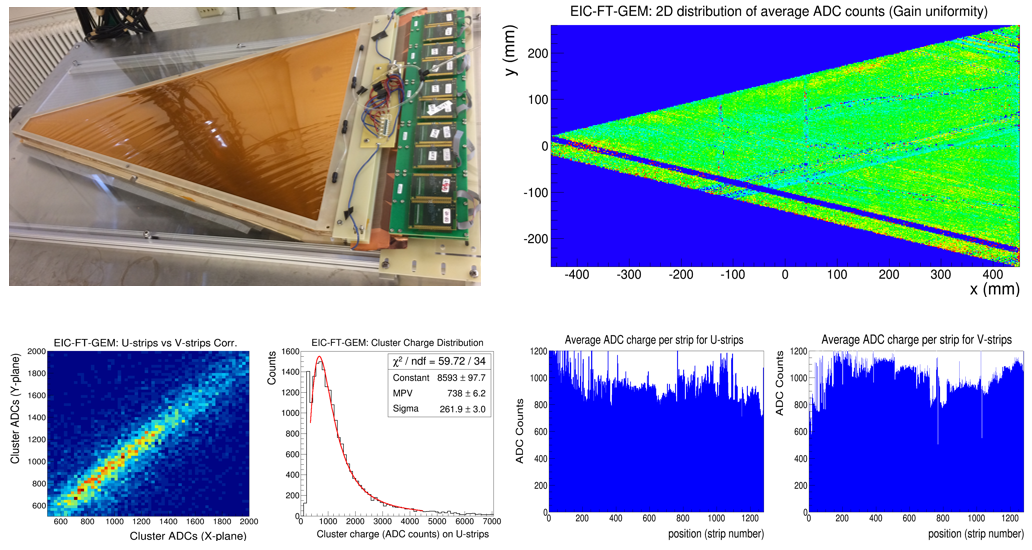
\includegraphics[width=1\columnwidth,trim={0pt 0mm 0pt 0mm},clip]{UVa_plots/eicCosmic}
\caption{\label{fig:eicCosmic}({\it Top left:}) EIC GEM prototype on the cosmic bench at UVa;  ({\it top right left:}) Gain uniformity: average charge (ADC counts) distribution over the active area; ({\it bottom from right to left:}) Charge sharing correlation between the top layer (U-strips) and bottom layer (V-strips); ADC charge distribution (ADC counts) on the top U-strips with the fit to Landau function;  Average charge (ADC counts) on  individual strip for U-strips and V-strips layers.}
\end{figure}
%
The prototype was characterized with cosmics for a three weeks period during which we collected 4M triggered cosmic events. Fig.~\ref{fig:eicCosmic}( {\it top left})  shows the detector on the cosmic stand  in the Detector Lab at UVa and basic characteristics plots.  The plot on {\it top right}, shows a fairly uniform distribution of the average ADC (ratio of the total accumulated charge over the total number of hits inside the area)  across  the active area for 4 millions cosmic event. This is a measure of the gain uniformity ac cross the chamber. The efficiency drops along the lines where the GEM support spacers can be clearly seen together broken strips and dead area.  These results successfully demonstrated   that the double-sided zebra connection scheme that we developed is working as expected. Very good  charge sharing  between the top layer (U-strips) and bottom layer (V-strips) of the U-V strips readout board  is shown on the charge correlation plot({\it bottom right}). The current U-V strips layer design is a clear improvement from the  one that we tested in the first prototype tested in 2013 \cite{Gnanvo:2015xda}. The  charge distribution (in ADC channels) of the top layer strip ({\it bottom center}) fit very nicely with the Landau function expected from the charge deposited by minimum ionizing particles. A good gain uniformity is also observed for the average ADC by each individual strips of the U and V strips layer respectively on the ({\it bottom center}) and  ({\it bottom right})  
%
%\paragraph*{Characterization of  $\mu$RWELL prototype with X-ray and $^{90}Sr$ sources:}\mbox{}\\
%We have completed the assembly of the meter-long low-mass Triple-GEM detector with \ang{30} stereo-angle U-V readout strip foil. The standard stretch-and-glue assembly technique was used for this prototype. Fig.~\ref{fig:uva_eic_gem_assembly} shows a couple of steps from this assembly process. The key points for the prototype relevant for EIC are:
%
%\begin{figure}[htb]
%\centering
%\includegraphics[width=1\columnwidth,trim={0pt 0mm 0pt 0mm},clip]{UVa_plots/uRwellXray}
%\caption{\label{fig:uRwellXray} ({\it Top left:}) Picture of the $\mu$RWELL structure on top of the 2D strip readout before final assembly. ({\it Top right:})  Cross section of $\mu$RWELL detector with 2D strip readout; ({\it Bottom left :}) Gain and efficiency curve ad a function of the electric field (E$_{Drift}$) in the drift; ({\it bottom center:}) Gain and efficiency curve as a function the electric field (E$_{{\mu}RWELL}$) in the  $\mu$RWELL structure; ({\it bottom right:}) Charge sharing correlation between the X-Y strips.}
%\end{figure}
%
\paragraph*{The prototypes in FTBF test beam at FNAL}\mbox{}\\
%
\begin{figure}[htb]
\centering
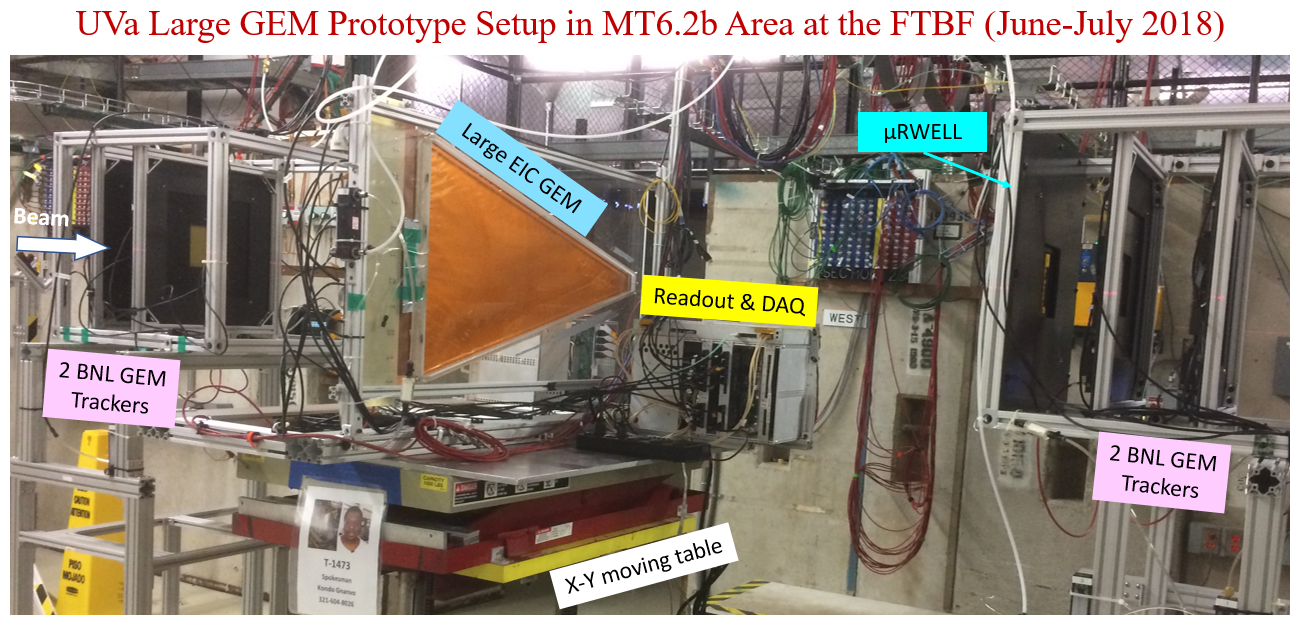
\includegraphics[width=1\columnwidth,trim={0pt 0mm 0pt 0mm},clip]{UVa_plots/ftbfSetup}
\caption{\label{fig:ftbfSetup} Setup of the large EIC GEM prototype on the moving X-Y table of MT6.2b area at the FTBF in June-July 2018, with two BNL GEMs for the upstream telescope and two other BNL GEMs combined our  small $\mu$RWELL prototype for the downstream telescope.}
\end{figure}
\begin{figure}[htb]
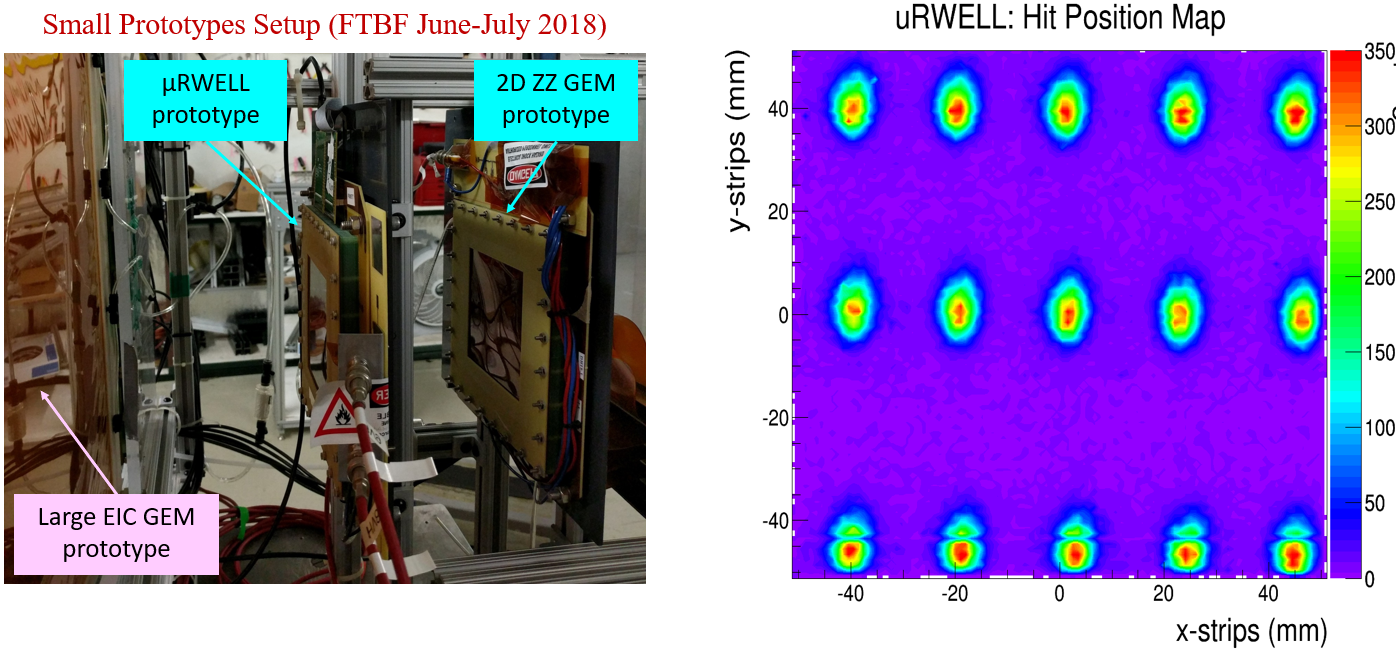
\includegraphics[width=1\columnwidth,trim={0pt 0mm 0pt 0mm},clip]{UVa_plots/ftbfSmallSetup}
\caption{\label{fig:ftbfSmallSetup} ({\it Left:}) The $\mu$RWELL prototype with 2D X-Y readout strip, the cross section of the detector is shown at the bottom; ({\it right:}) Setup of $\mu$RWELL  prototype and a small triple-GEM prototype with 2D zigzag strip readout at the FTBF in June-July 2018. The prototypes were installed on the same moving table behind the large EIC GEM.}
\end{figure}
%
The large EIC GEM prototype, the $\mu$RWELL prototype  and an additional small triple-GEM with 2D zigzag strip prototypes were brought to the Fermilab Test Beam Facility (FTBF) this summer (June 2018 - July 2018) for a period of 3 weeks and tested with the 120 GeV primary proton beam. The beam test campaign was a combined effort which includes M. Hohlmann's group  from Florida Tech (FIT), also testing  their large EIC GEM prototype with zigzag strip readout and K. Dehmelt and T. Hemmick's group from Stony Brook (SBU) testing their small TPC prototype with GEM readout. UVa and FIT shared the same large EIC GEMs setup with the prototypes installed on the X-Y moving table of the  MT6.2b area at the FTBF. For the tracking, our colleagues from BNL group provided four small triple-GEMs COMPASS readout. The setup is shown on  Fig.~\ref{fig:ftbfSetup}  with the four BNL GEMs and the $\mu$RWELL prototype used as upstream and downstream telescope. The detector configuration in the setup  was optimized to minimize the  multiple scattering impact on the resolution studies of the EIC GEM prototype. In addition, we also had a second detector configuration setup dedicated to a short study (one day beam time) of the small  $\mu$RWELL and the 2D zigzag GEM prototypes. In this second setup, the two small detectors were installed on the X-Y moving table behind the large EIC prototype as shown on Fig.~\ref{fig:ftbfSmallSetup}. All chambers, including the four BNL GEM trackers operated with the same Ar-CO2 (70/30) gas mixture and the same APV25-based Scalable Readout System (SRS) developed at CERN by the RD51 collaboration were used to read out all chambers. DATE and AMORE (developed by the CERN ALICE experiment) where used respectively as DAQ software and online/offline data analysis tool. The FTBF coincidence scintillators signal was used to trigger the DAQ at a rate of $\sim$ 400Hz.\\
%
\begin{figure}[htb]
\centering
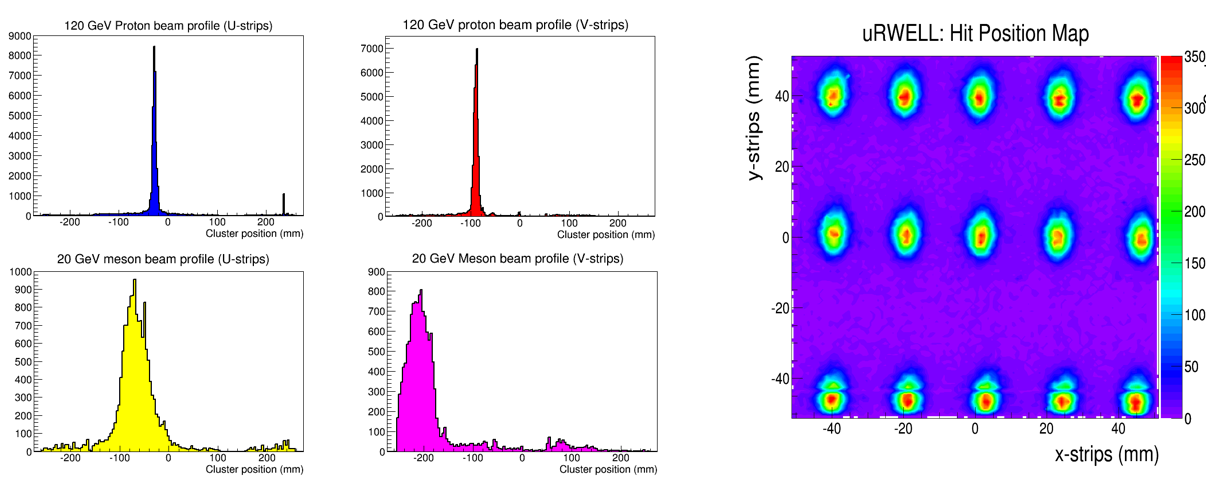
\includegraphics[width=1\columnwidth,trim={0pt 0mm 0pt 0mm},clip]{UVa_plots/ftbfBeamPosScan}
\caption{\label{fig:ftbfBeamPosScan} ({\it Left:}) 1D beam profile, in the large EIC GEM prototype, of 120 GeV proton (top) and 20 GeV meson beam (bottom) top and bottom U-V strips readout layer. ({\it Right:}) 2D beam spot reconstruction of 120 GeV proton beam from position scan in the $\mu$RWELL prototype.}
\end{figure}
%
Fig.~\ref{fig:ftbfBeamPosScan} shows a few examples FTBF hadron beams profile in the large  EIC GEM prototype the 2D spot from beam position scan in $\mu$RWELL prototype. The horizontal line split for the spots at the bottom of the plots of the $\mu$RWELL are caused a few broken strips of the X-Y strips readout board.
%
\paragraph*{Production quality issues with the EIC U-V strips readout foil:}\mbox{}\\
\begin{figure}[htb]
\centering
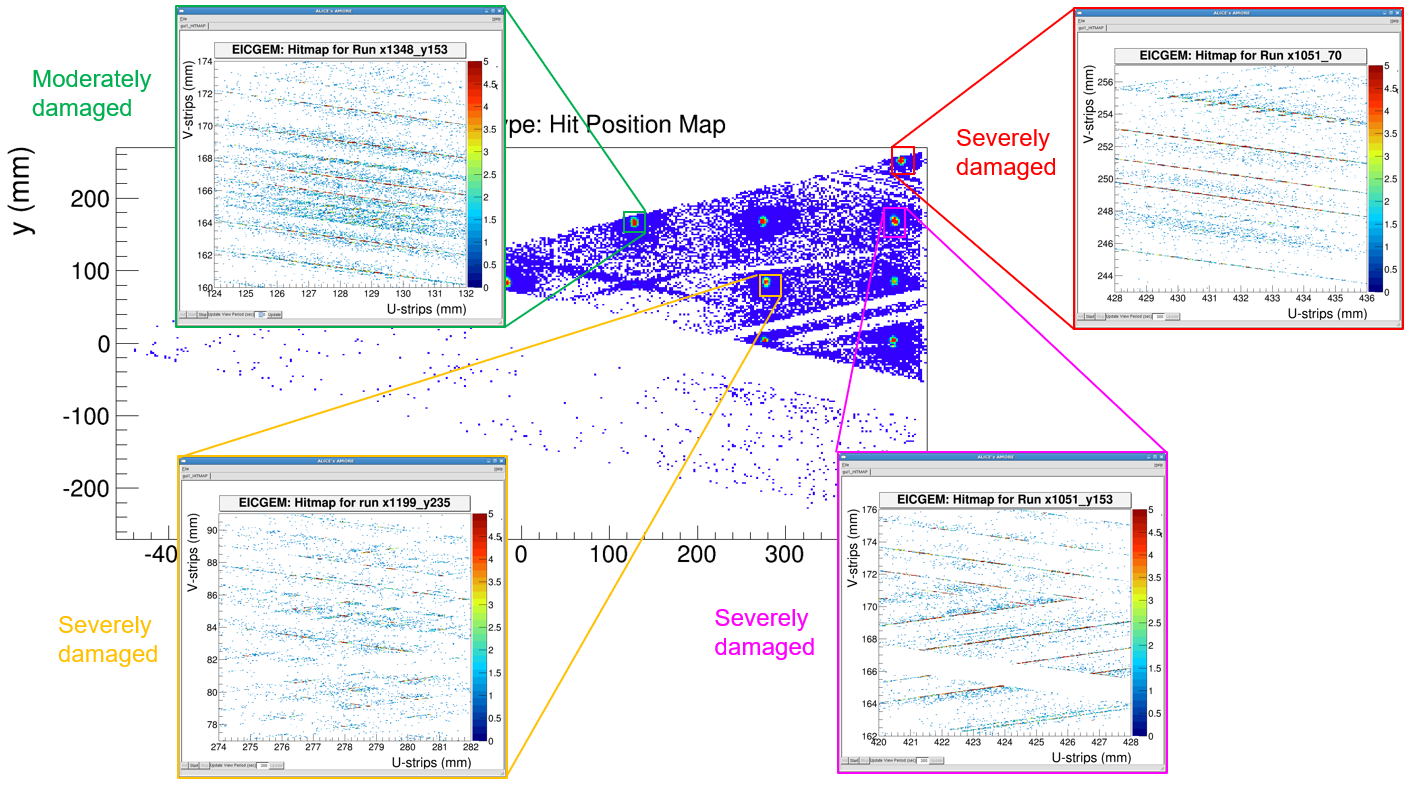
\includegraphics[width=1\columnwidth,trim={0pt 0mm 0pt 0mm},clip]{UVa_plots/eicPosScan}
\caption{\label{fig:eicPosScan}  2D  reconstruction of 120 GeV proton beam from position scan in the top half of the EIC GEM prototype. A zoom in of  reconstructed particle positions for at four beam spots showing some unexpected patterns of non uniform distribution of the reconstructed particle positions likely due to poor production quality of the readout strip layer.}
\end{figure}
Fig.~\ref{fig:eicPosScan} shows the 2D proton beam reconstruction from a position scan run in the large EIC GEM prototype. A closer look (very fine histogram binning) at the reconstructed beam position  reveals some unexpected patterns for reconstructed positions as shown on  four beam spot locations on the plots. We normally expect an uniform distribution of the reconstructed points. Instead, what we actually observed for most of the beam spot is a reconstructed positions heavily concentrated along a set of line parallel to the strips. As indicated on the plots of Fig.~\ref{fig:eicPosScan}, the discrete pattern of the reconstructed positions is more or less pronounced in some locations than  other but seems to be present anywhere where we were able to collect data from. This pattern suggests the possibility of a significant number shorts between the strips in both the top and bottom strip layers. A few consecutive shorted strips will results in  large hit signal replicated on several FE channels connected to these strips that would make it impossible to extract the  position information with good accuracy through the charge centroid approach. The test beam data  seem to confirm that hypothesis. Another possible explanation could be some issue with the signal quality extracted from the zebra strips that interface the detector readout strips to the FE electronic channel. Short contacts could potentially originate from the zebra strips or from the Panasonic-to-Zebra PCB adapter that we use in these scheme. We are investigating this  problem with some ongoing tests in the lab.
%
\paragraph*{Track fit residuals analysis}\mbox{}\\
%
\begin{enumerate}
\item \textbf{Performances of BNL GEM trackers:}
%
\begin{figure}[htb]
\centering
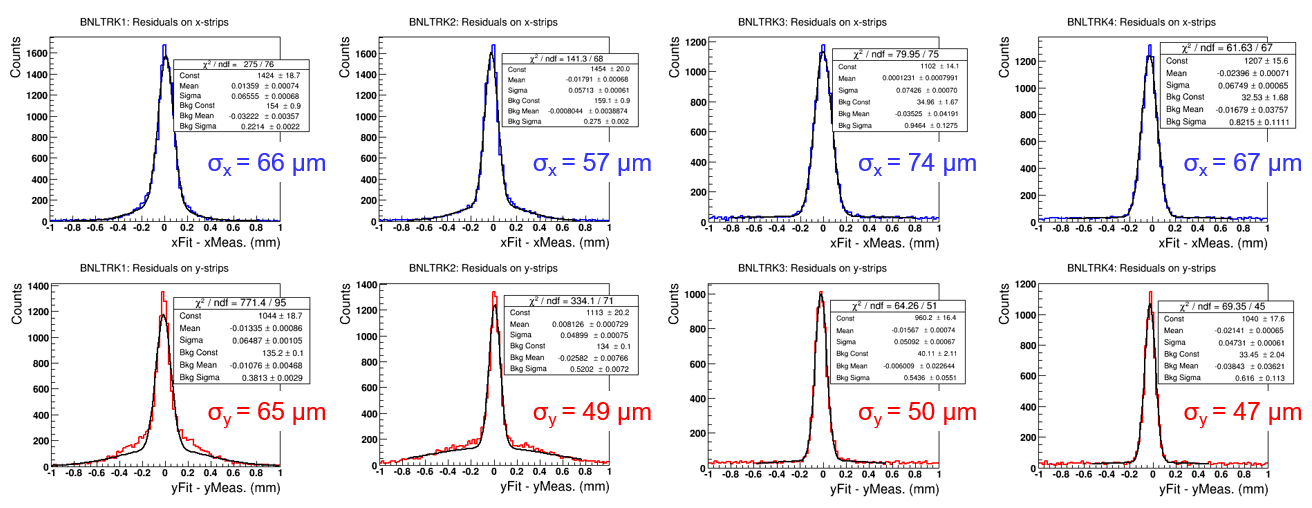
\includegraphics[width=1\columnwidth,trim={0pt 0mm 0pt 0mm},clip]{UVa_plots/trkResidual}
\caption{\label{fig:trkResidual} Residual distribution in x and y of BNL GEM trackers with the 120 GeV proton beam.}
\end{figure}
We  just started looking the spatial resolution analysis for the large EIC prototype as well as the small prototypes that were tested at Fermilab. The first step was the production of the offsets parameters in x-y plane perpendicular to the beam direction z for both the trackers (BNL GEMs) and the prototypes under test. For all the residual distribution results reported below, the x and y offset correction were performed and applied, however the z position of the detector setup at the FTBF were just measured manually and software correction of the z position has not yet been implemented. 

Fig.~\ref{fig:trkResidual} shows the residual distribution in x and y for each of the 4 BNL GEM trackers with the 120 GeV proton beam data. The distribution for each tracker is obtained from least squares fit of straight line track  by four space point coordinates of the 3 other BNL GEM trackers and the $\mu$RWELL prototype. The large variation of the width (sigma) of the residual distribution  from one tracker to  the other can be explained by the detector were not operating at the same effective gain during the test beam even though the same voltage was applied to the divider. Also the distribution are residual and not the detector resolution since we did not yet correct for the track fit error which we would expect would lower the sigma value by $\sim$10 $\mu$m for each plot. 

\item \textbf{Large EIC GEM prototype:}
\begin{figure}[htb]
\centering
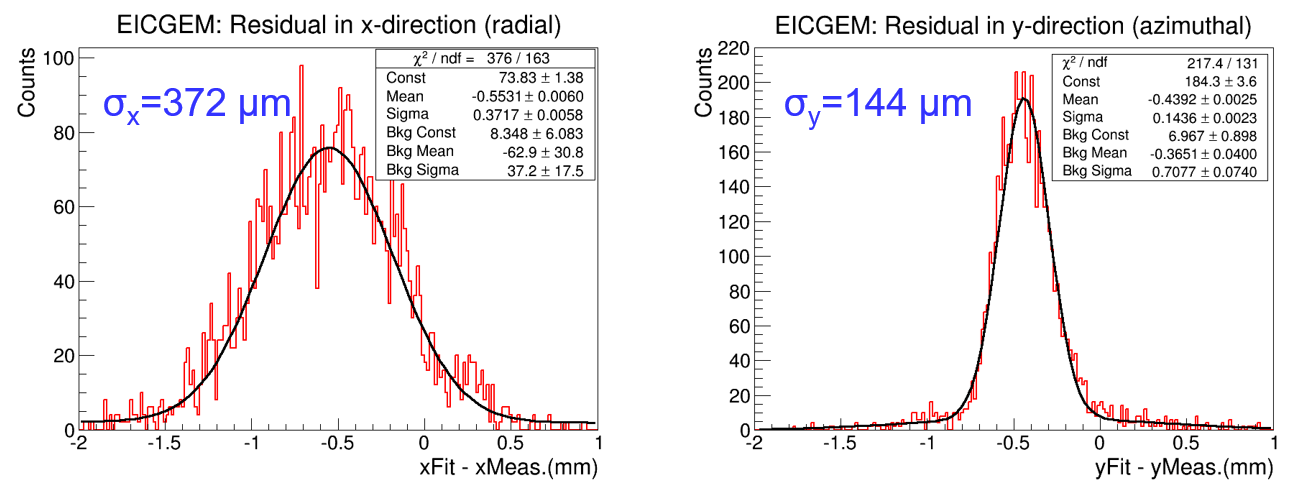
\includegraphics[width=1\columnwidth,trim={0pt 0mm 0pt 0mm},clip]{UVa_plots/eicResidual}
\caption{\label{fig:eicResidual} Residuals in x and y of the EIC GEM prototype with the 120 GeV FTBF proton beam.}
\end{figure}
%
completed the assembly of the meter-long low-mass Triple-GEM detector with \ang{30} stereo-angle U-V readout strip foil. The standard stretch-and-glue assembly technique was used for this prototype. Fig.~\ref{fig:uva_eic_gem_assembly} shows a couple of steps from this assembly process. The key points for the prototype relevant for EIC are:
%
\item \textbf{$\mu$RWELL prototype:}
%
For this Triple-GEM prototype, we use only foils including for the drift cathode and the U-V strips readout board, with no rigid PCB or support structure  in the active area. The 2D U-V strips readout layer and the drift cathode were all produced at CERN from the same copper clad Kapton base material used for the production of GEM foils.The elimination of rigid support structure in the active area of the detector is motivated by for low material requirement to minimize multiple scattering as well as photon induced background. Entrance and exit gas volume with 25 $\mu$m thick Kapton foil have been added to the stack of active foils for pressure balance inside the chamber in order to maintain uniform gap between different layers needed for an uniform gain across the active area.  Top left picture of Fig.~\ref{fig:uva_eic_gem_assembly} shows a cross section of the all foils EIC-FT-GEM prototype with the entrance and exit gas windows.
%
\begin{figure}[htb]
\centering
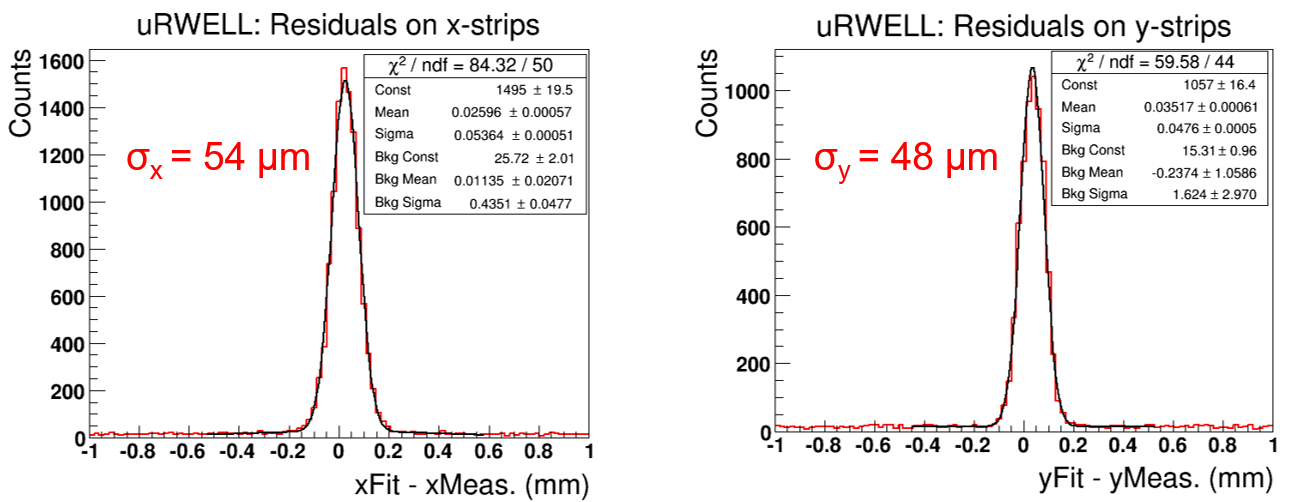
\includegraphics[width=1\columnwidth,trim={0pt 0mm 0pt 0mm},clip]{UVa_plots/uRwellResidual}
\caption{\label{fig:uRwellResidual} Residuals in x and y of the $\mu$RWELL prototype with the 120 GeV FTBF proton beam.}
\end{figure}
%
\end{enumerate}
